% Seção: Estrutura geral de compiladores e interpretadores

\section{Estrutura geral de compiladores e interpretadores}
\label{revisao:estrutura-geral}

Na figura \ref{fig:compilador} h\ah\ um esquema do funcionamento geral de um compilador, que segundo \cite{Aho08}, recebe como entrada um programa em uma linguagem de programa\ca o - a linguagem \emph{fonte} - e traduz para um programa equivalente em outra linguagem - a linguagem \emph{objeto}.

Um exemplo de interpretador pode ser visto na figura \ref{fig:interpretador}.

\begin{figure}[htp]
  \begin{center}
    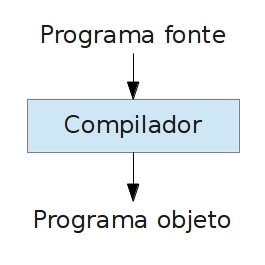
\includegraphics[width=0.25\textwidth]{figuras/compilador}
  \end{center}
  \caption{Estrutura de um compilador}
  \label{fig:compilador}
\end{figure}

\begin{figure}[htp]
  \begin{center}
    
\includegraphics[width=0.6\textwidth]{figuras/interpretador}
  \end{center}
  \caption{Estrutura de um interpretador}
  \label{fig:interpretador}
\end{figure}

Internamente, ambos os programas s\ao\ semelhantes, como explica \cite{Aho08}, a seguir.

\subsection{An\ah lise l\eh xica}

Segundo \cite{Aho08}, o analisador l\eh xico \eh\ o primeiro passo de um compilador. Ele \eh\ respons\ah vel pela leitura dos caracteres de entrada (o programa fonte), discartando coment\ah rios e espa\cc os em branco, produzindo uma sequ\^encia de \emph{tokens} ou lexemas que ser\ao\ consumidos pelo analisador sem\^antico.

Outra atividade do analisador l\eh xico \eh\ correlacionar as mensagens de erro encontradas pelo compilador como um todo, a localiza\co es no programa fonte original.

% -- Express\oe s regulares ?

% -- Diagramas de transi\ca o ?

Uma das ferramentas que auxiliam na gera\ca o do analisador l\eh xico \eh\ o Lex, ou sua implementa\ca o mais recente, o Flex.

\cite{Niemann10} descreve o Lex como uma ferramenta que l\^e uma entrada e a converte em tokens, segundo um padr\ao, que pode ser expresso atrav\eh s de express\oe s regulares. Cada padr\ao, \eh\ associado a uma a\ca o, que geralmente retorna a sequ\^encia encontrada para o analisador sint\ah tico.

Dependendo da gram\ah tica da linguagem, podem ocorrer conflitos entre pad\oe s de lexemas, e, segundo \cite{Aho08}, o Lex toma basicamente duas regras para sua resolu\ca o:

\begin{enumerate}
\item Preferir tokens mais longos aos mais curtos
\item Opte pelo padr\ao\ descrito primeiro, no caso de um prefixo combinar com mais de um padr\ao.
\end{enumerate}

Uma das t\eh cnicas para evitar os conflitos, segundo \cite{Aho08}, \eh\ a utiliza\ca o do caractere de \emph{lookahead}, que indica a pr\oh ximo caractere na entrada.

O Lex, segundo \cite{Aho08}, funciona a partir da implementa\ca o de um aut\^omato finito, isto \eh, grafos ou diagramas de transi\ca o que dizem se uma entrada atende a um padr\ao\ ou n\ao, e que podem ser determin\ih sticos (quando cada s\ih mbolo ou caractere expressa apenas uma transi\ca o\footnote{Transi\ca o, aresta ou sa\ih da s\ao sin\^onimos neste contexto.} de um estado para outro) ou n\ao-determin\ih sticos (quando um s\ih mbolo pode rotular mais de uma transi\ca o.). Ambos podem ser descritos atrav\eh s de linguagens regulares, como express\oe s regulares. \cite{Niemann10} completa afirmando que qualquer express\ao\ regular pode ser expressa em um aut\^omato finito\footnote{N.A. Traduzido pelo autor.}.

% -- Seria necess\ah rio demonstrar a estrutura de um analisador l\eh xico j\ah\ neste documento ?

\subsection{An\ah lise sint\ah tica}

\cite{Aho08} afirma que as linguagens possuem formas precisas de descrever suas estruturas sint\ah ticas, ou seja, a forma como as palavras-chave e s\ih mbolos s\ao\ dispostos no c\oh digo fonte.

Ele ainda afirma que a especifica\ca o da gram\ah tica facilita a compreens\ao\ da linguagem de programa\ca o, permite que o analisador sint\ah tico seja gerado automaticamente, facilita a tradu\ca o do programa e detec\ca o de erros, al\eh m de permitir que a linguagem seja constru\ih da iterativamente.

O analisador sint\ah tico, segundo \cite{Aho08}, tem papel de receber a sequ\^encia de tokens do analisador l\eh xico, verificando se pertence \`a gram\ah tica, emitindo erros no caso da sequ\^encia n\ao\ combinar.

Sua estrat\eh gia de funcionamento geralmente s\ao\ ascendente (bottom-up) ou descendente (top-down). A estrat\eh gia ascendente constr\oh i a \ah rvore que representa o c\oh digo da ra\ih z para as folhas\footnote{Imagine uma \ah rvore de ponta-cabe\cc a.}, enquanto a descendente faz vice-versa.

As subclasses LL e LR\footnote{-- Incluir explica\ca o sobre as diferen\cc as entre as duas.} s\ao\ as expressivas o suficientes para a maioria das gram\ah ticas, segundo \cite{Aho08}.

% -- Explica\ca o sobre gram\ah ticas livres de contexto

% -- Ambig\"uidade na gram\ah tica

% -- Analisador ascendente (LR)

% -- An\ah lise Shift-Reduce

% -- LALR (Look-ahead)

% -- Preced\^encia e associatividade

% -- Yacc

\subsection{An\ah lise sem\^antica}

Segundo \cite{Aho08}, \eh durante a etapa de an\ah lise sem\^antica que, utilizando a \ah rvore sint\ah tica e a tabela de s\ih mbolos, ocorrem as verifica\co es de consist\^encia do programa, entre elas a coer\ca o de tipos, verifica\ca o est\ah tica de erros e otimiza\ca o sem\^antica.

Na verifica\ca o de tipos as declara\co es de m\eh todos e vari\ah veis s\ao\ avaliados para confirmar se combinam com os tipos dos resultados das express\oe s e comandos utilizados no programa. Por exemplo, o analisador sem\^antico pode alertar sobre a tentativa de somar um dado do tipo inteiro (\emph{int}) com um dado do tipo texto (\emph{string})\footnote{Tal opera\ca o pode resultar em erros de mem\oh ria e falha do programa.}.

Na verifica\ca o est\ah tica s\ao\ rastreados erros que podem ocorrer em tempo de execu\ca o do programa, como utiliza\ca o de vari\ah veis que n\ao\ tem valor definido (valor nulo) e tentativa de divis\ao\ por zero.

Na otimiza\ca o sem\^antica, um determinado conjunto de instru\co es pode ser reduzido por outro menor e equivalente, ou seja, ocorre a redu\ca o de instru\co es sem que haja detrimento das opera\co es realizadas.

\subsection{Gera\ca o de c\oh digo intermedi\ah rio}
\label{revisao:estrutura-geral:geracao-codigo}

Segundo \cite{Aho08}, no modelo de s\ih tese e an\ah lise de um compilador, o \emph{front-end} analisa o programa fonte e gera uma representa\ca o intermedi\ah ria, a partir da qual o \emph{back-end} gera o c\oh digo objeto. O esfor\cc o de constru\ca o de compiladores pode ser reduzido separando-se os detalhes da linguagem de programa\ca o no \emph{front-end} e os detalhes do c\oh digo objeto da m\ah quina alvo no \emph{back-end}. Com isso, torna-se poss\ih vel construir \(m \times n\) conjuntos de compiladores, construindo-se apenas \emph{m front-ends} e \emph{n back-ends}, j\ah\ que o ponto de compatibilidade entre os dois componentes \eh\ a especifica\ca o da representa\ca o intermedi\ah ria.

\cite{Aho08} aborda a estrat\eh gia de tr\^es endere\cc os, onde cada instru\ca o do programa fonte \eh\ dividida em uma sequ\^encia de instru\co es com no m\ah ximo um operador e tr\^es argumentos\footnote{Esta \eh\ a mesma abordagem utilizada na \emph{LLVM-IR}, conforme ser\ah\ discutido na se\ca o \ref{llvm:llvm-ir}}, na forma \( v1 = v2 \mbox{ \bf{op} } v3 \), onde v1, v2 e 3 s\ao\ vari\ah veis e \emph{op} \eh\ o operador aplicado. Existem instru\co es adicionais para o fluxo de controle, como estruturas de decis\ao\ e estruturas de repeti\ca o.

Segundo \cite{Aho08} a atribui\ca o \uh nica est\ah tica (SSA\sigla{SSA}{Do ingl\^es \emph{Static Single-Assignment}}, do ingl\^es \emph{Static Single-Assignment}, desenvolvida inicialmente por \cite{Cytron91}), \eh\ uma forma de representa\ca o em que as vari\ah veis do c\oh digo intermedi\ah rio de tr\^es endere\cc os possuem nomes distintos e que seu valor nunca \eh\ alterado, facilitando certas otimiza\co es, conforme veremos na se\cc \ao\ \ref{estrutura-geral:otimizacao}. Abaixo um exemplo da forma SSA:

{\renewcommand{\arraystretch}{0.8}

\begin{table}[htbp]\footnotesize
\begin{center}
\begin{tabular}{p{5cm} p{4cm} p{5cm}}
\begin{tabular}{p{3cm}} \begin{verbatim}
p = a + b
q = p - c
p = q * d
p = e - p
q = p + q
\end{verbatim} \\ \end{tabular} \caption{C\oh digo de tr\^es endere\cc os} &  & \begin{tabular}{p{3cm}} \begin{verbatim}
p1 = a + b
q1 = p1 - c
p2 = q1 * d
p3 = e - p2
q2 = p3 + q1
\end{verbatim} \\ \end{tabular} \caption{Forma de atribui\ca o \uh nica est\ah tica}
\end{tabular}
\end{center}
\end{table}

} \quad

Dada a representa\ca o intermedi\ah ria, novas otimiza\co es podem ser aplicadas ao c\oh digo, reduzindo a quantidade de instru\co es por comando. Algumas instru\co es podem inclusive ser removidas sem perda de sentido sem\^antico. Podem ser necess\ah rias v\ah rias passadas pela fase de otimiza\ca o antes da gera\ca o do c\oh digo objeto, conforme explica \cite{Aho08}.

\subsection{Otimiza\ca o da representa\ca o intermedi\ah ria}
\label{estrutura-geral:otimizacao}

Segundo \cite{Aho08}:

\begin{citacao}
A elimina\ca o de instru\co es desnecess\ah rias no c\oh digo objeto, ou a substitui\ca o de uma sequ\^encia de instru\co es por uma sequ\^encia mais r\ah pida, que efetua a mesma opera\ca o, usualmente \eh\ denominada 'melhoria do c\oh digo' ou 'otimiza\ca o do c\oh digo'.
\end{citacao}

Tal melhoria \eh\ baseada na \emph{an\ah lise de fluxo de dados}, que difere de acordo com o contexto. Por exemplo, a an\ah lise de constantes verifica os locais em que a constante \eh\ utilizada, ponderando se \eh\ poss\ih vel substituir a refer\^encia (nome) da constante pelo seu valor. J\ah\ a an\ah lise de tempo de vida, determina se uma vari\ah vel com certeza tem seu valor alterado antes de ser utilizado, evitando a necessidade de mant\^e-la na mem\oh ria.

Podemos ver no exemplo abaixo, retirado da obra de \cite{Aho08}, uma transforma\ca o de c\oh digo intermedi\ah rio sem perda de sem\^antica.

{\renewcommand{\arraystretch}{0.8}
\begin{table}[htbp]\footnotesize
\begin{center}
\begin{tabular}{p{6cm} p{2cm} p{6cm}}
\begin{tabular}{|p{4cm}|} \hline \begin{verbatim}
B5:
  t6 = 4 * i
  x = a[t6]
  t7 = 4 * i
  t8 = 4 * j
  t9 = a[t8]
  a[t7] = t9
  t10 = 4 * j
  a[t10] = x
  goto B2
\end{verbatim} \\ \hline \end{tabular} \caption{Antes da otimiza\ca o} &  & \begin{tabular}{|p{4cm}|} \hline \begin{verbatim}
B5:
  t6 = 4 * i
  x = a[t6]
  t8 = 4 * j
  t9 = a[t8]
  a[t6] = t9
  a[t8] = x
  goto B2
\end{verbatim} \\ \hline \end{tabular} \caption{Depois da otimiza\ca o}
\end{tabular}
\end{center}
\end{table}
} \quad

Outro exemplo de otimiza\ca o simples \eh\ a propaga\ca o por c\oh pia, na qual os desvios condicionais do programa s\ao\ desdobrados, de tal forma que, dada uma express\ao\ \emph{variavel = valor}, copia-se \emph{valor} para todas as localiza\co es em que \emph{variavel} \eh\ lida, at\eh\ que seu valor seja novamente alterado, passando seu novo valor da mesma forma.

O objetivo desse processo fica claro quando verificamos o pr\oh ximo exemplo de otimiza\ca o, a remo\ca o do c\oh digo morto ou inalcan\cc \ah vel, quando uma determinada sequ\^encia de instru\co es n\ao\ ser\ah\ utilizada em tempo de execu\ca o. Sabendo-se o valor que leva at\eh\ tal conjunto de instru\co es, fica f\ah cil para o compilador deduzir que este c\oh digo n\ao\ ser\ah\ utilizado, conforme explica \cite{Aho08}.

Segundo \cite{Aho08}, os dois primeiros compiladores que fizeram otimiza\co es mais extensas forma Alpha \cite{Ershov66} e Fortran H \cite{Lowry69}.

\subsection{Gera\ca o de c\oh digo objeto}

Segundo \cite{Aho08}, a gera\ca o de c\oh digo objeto \eh\ a fase final do compilador, onde cada instru\ca o da representa\ca o intermedi\ah ria (que j\ah\ passou pelas transforma\co es e otimiza\co es necess\ah rias) \eh\ mapeada para instru\co es da linguagem objeto.

Este processo inclui a sele\ca o de instru\co es, aloca\ca o e atribui\ca o de registradores, que est\ao\ fortemente relacionados \`a arquitetura da m\ah quina alvo, como por exemplo as diferen\cc as entre as m\ah quinas CISC e RISC.

% \subsection{Ambiente de execu\ca o}

% -- Necessário?

\subsection{JIT - Compila\ca o \emph{Just-in-Time}}

Segundo \cite{wiki:jit}, JIT\sigla{JIT}{Do ingl\^es, compila\ca o \emph{Just-in-Time}}, \eh\ um compilador que traduz de um formato para outro, por exemplo, bytecode para c\oh digo de m\ah quina.

Isso permite, em tempo de execu\ca o, que o software ganhe desempenho em ponto cr\ih ticos e gargalos.
